\section{Recap}%
\label{sec:recap}

\begin{frame}
	\frametitle{Previously on TI1520TW}
	\begin{center}
		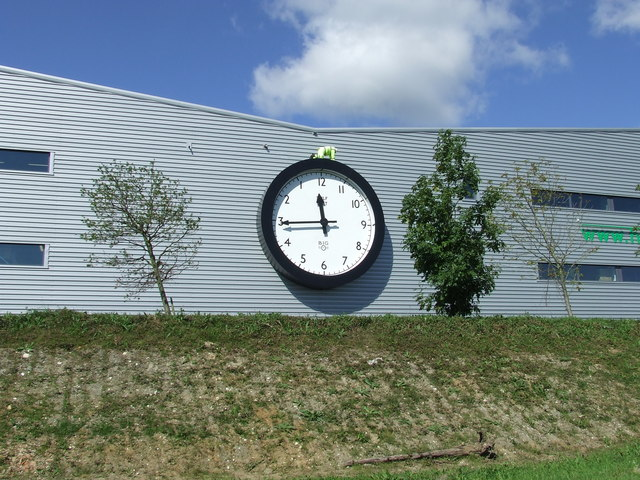
\includegraphics[width=0.8\textwidth]{figures/clock.jpg}\\
		\hspace*{15pt}\hbox{\scriptsize Image By:\thinspace{\itshape Keith Evans}}
		% https://www.geograph.org.uk/photo/548627
	\end{center}
	
\end{frame}

\begin{frame}
	\frametitle{Recap of Maps}
	
	\begin{center}
		\begin{tabular}{c | c | c}
			Operation & Expected Time & Worst-case \\
			\midrule
			\texttt{M.size()} & $\Theta(1)$& $\Theta(1)$\\
			\texttt{M.get(k)}  & $\Theta(1)$& $\Theta(n)$\\
			\texttt{M.put(k,v)} & $\Theta(1)$& $\Theta(n)$\\
			\texttt{M.remove(k)} & $\Theta(1)$& $\Theta(n)$\\
			\texttt{M.contains(k)} & $\Theta(1)$& $\Theta(n)$\\
		\end{tabular}
	\end{center}
		\begin{block}{What does this depend on?}
			It all stands or falls with the hash function!
			\begin{itemize}
				\item Fewer hash-conflicts means better performance.
				\item Separate chaining or (linear) probing does not matter for time performance.
				\item The latter saves us some space, but is not better in terms of space or time \textit{complexity}.
			\end{itemize}
		\end{block}	
\end{frame}

\begin{frame}
	\frametitle{Recap of Trees}
	\begin{columns}
		\column{0.405\textwidth}
			\begin{tikzpicture}[
				level distance = 2.5em,
				level 1/.style={sibling distance=9em},
				level 2/.style={sibling distance=4.5em},
				level 3/.style={sibling distance=2.25em},
			]
			\node[ellipse] (t1) {root}
				child { node[ellipse] {child 1}
					child { node[ellipse] {leaf 1}}
				}
				child { node[ellipse] {child 2}
					child { node[ellipse] {leaf 2}}
					child { node[ellipse] {leaf 3}}
					child { node[ellipse] {leaf 4}}
				};
			\end{tikzpicture}
		\column{0.555\textwidth}
		\begin{itemize}
			\item The \textit{root node} is the node that has no \textit{parent}.
			\item A node can have \textit{children}.
			\item A node without children is called a \textit{leaf}.
			\item Two nodes with the same \textit{parent} are \textit{siblings}.
			\item \textit{Descendants} are found by repeatedly following child-relations.
			\item \textit{Ancestors} are found by repeatedly following parent-relations.
		\end{itemize}
	\end{columns}
\end{frame}


